\chapter{Análise de viabilidade}

Para que uma solução tecnológica apresente potencial real de implantação, não basta considerar apenas sua execução técnica, sendo igualmente necessário avaliar sua aceitação pelo público, seus custos operacionais, sua capacidade de crescimento e as condições regulatórias envolvidas em sua operação. A análise de viabilidade busca verificar se uma solução de assistência financeira inteligente, preditiva e conversacional apresenta aderência às necessidades do público-alvo e condições para ser desenvolvida e mantida de maneira economicamente sustentável.

O EIGAM foi concebido para funcionar em qualquer ferramenta de conversa, sem depender de um serviço de mensageria específico, o que foi verificado com dois mensageiros de mercado e com uma conversa no painel \textit{web}. Além disso, a solução depende da integração com serviços externos, como provedores de inteligência artificial, de mensageria, de pagamento e de acesso ao ecossistema de \textit{Open Finance}. Dessa forma, a análise considera a aceitação da proposta, sua posição em relação às soluções concorrentes e os custos, riscos e requisitos envolvidos em sua implantação e expansão.
\section{Análise de demanda}

De acordo com Iunes (1995), a demanda pode ser definida como a relação direta entre a quantidade de determinado bem ou serviço que os consumidores desejam obter e o seu poder aquisitivo em um dado período. Dessa forma, a análise de demanda permite compreender necessidades, comportamentos e expectativas do público, contribuindo para avaliar a aderência de uma proposta ao mercado em que pretende atuar.

Com o objetivo de obter indícios sobre a aderência da solução proposta, foi aplicado um questionário quantitativo destinado a identificar dificuldades relacionadas à gestão financeira pessoal, o interesse por funcionalidades de assistência financeira baseadas em inteligência artificial, a familiaridade com o ecossistema de \textit{Open Finance} e a aceitação do \textit{WhatsApp} como canal inicial de interação.

O questionário, cujas questões são detalhadas no Apêndice A, foi respondido por 42 participantes entre 06 e 20 de abril de 2026, por meio da ferramenta Google Forms. O perfil predominante dos respondentes foi composto por adultos entre 25 e 44 anos, com ensino superior completo ou incompleto, distribuídos entre os sexos feminino (22), masculino (19) e um participante que preferiu não declarar. O detalhamento completo das respostas encontra-se na Tabela \ref{tab:questionario}, no Apêndice B.

Inicialmente, foi possível constatar que o \textit{WhatsApp} faz parte do cotidiano de praticamente todos os respondentes, uma vez que 41 dos 42 participantes (97,6\%) afirmaram utilizá-lo diariamente. Esse resultado fornece indícios favoráveis para sua adoção como primeiro canal de interação com o EIGAM, permitindo que a validação inicial do produto ocorra em um aplicativo já familiar à maior parte da amostra. Entretanto, esse dado não implica que a solução deva permanecer restrita a esse canal, razão pela qual sua arquitetura foi preparada para integrar outros serviços de mensageria.

Em relação aos hábitos financeiros, o gráfico da Figura \ref{fig:pq_frequencia} demonstra que a consulta ao saldo bancário é frequente: 22 respondentes (52,4\%) afirmaram realizá-la diariamente e 11 (26,2\%) de duas a três vezes por semana. Os resultados indicam que o acompanhamento das finanças já constitui uma atividade recorrente para parcela significativa da amostra, ainda que dependa predominantemente da iniciativa do próprio usuário.

\begin{figure}[H]
    \centering
    \caption{Frequência de consulta ao saldo bancário pelos respondentes}
    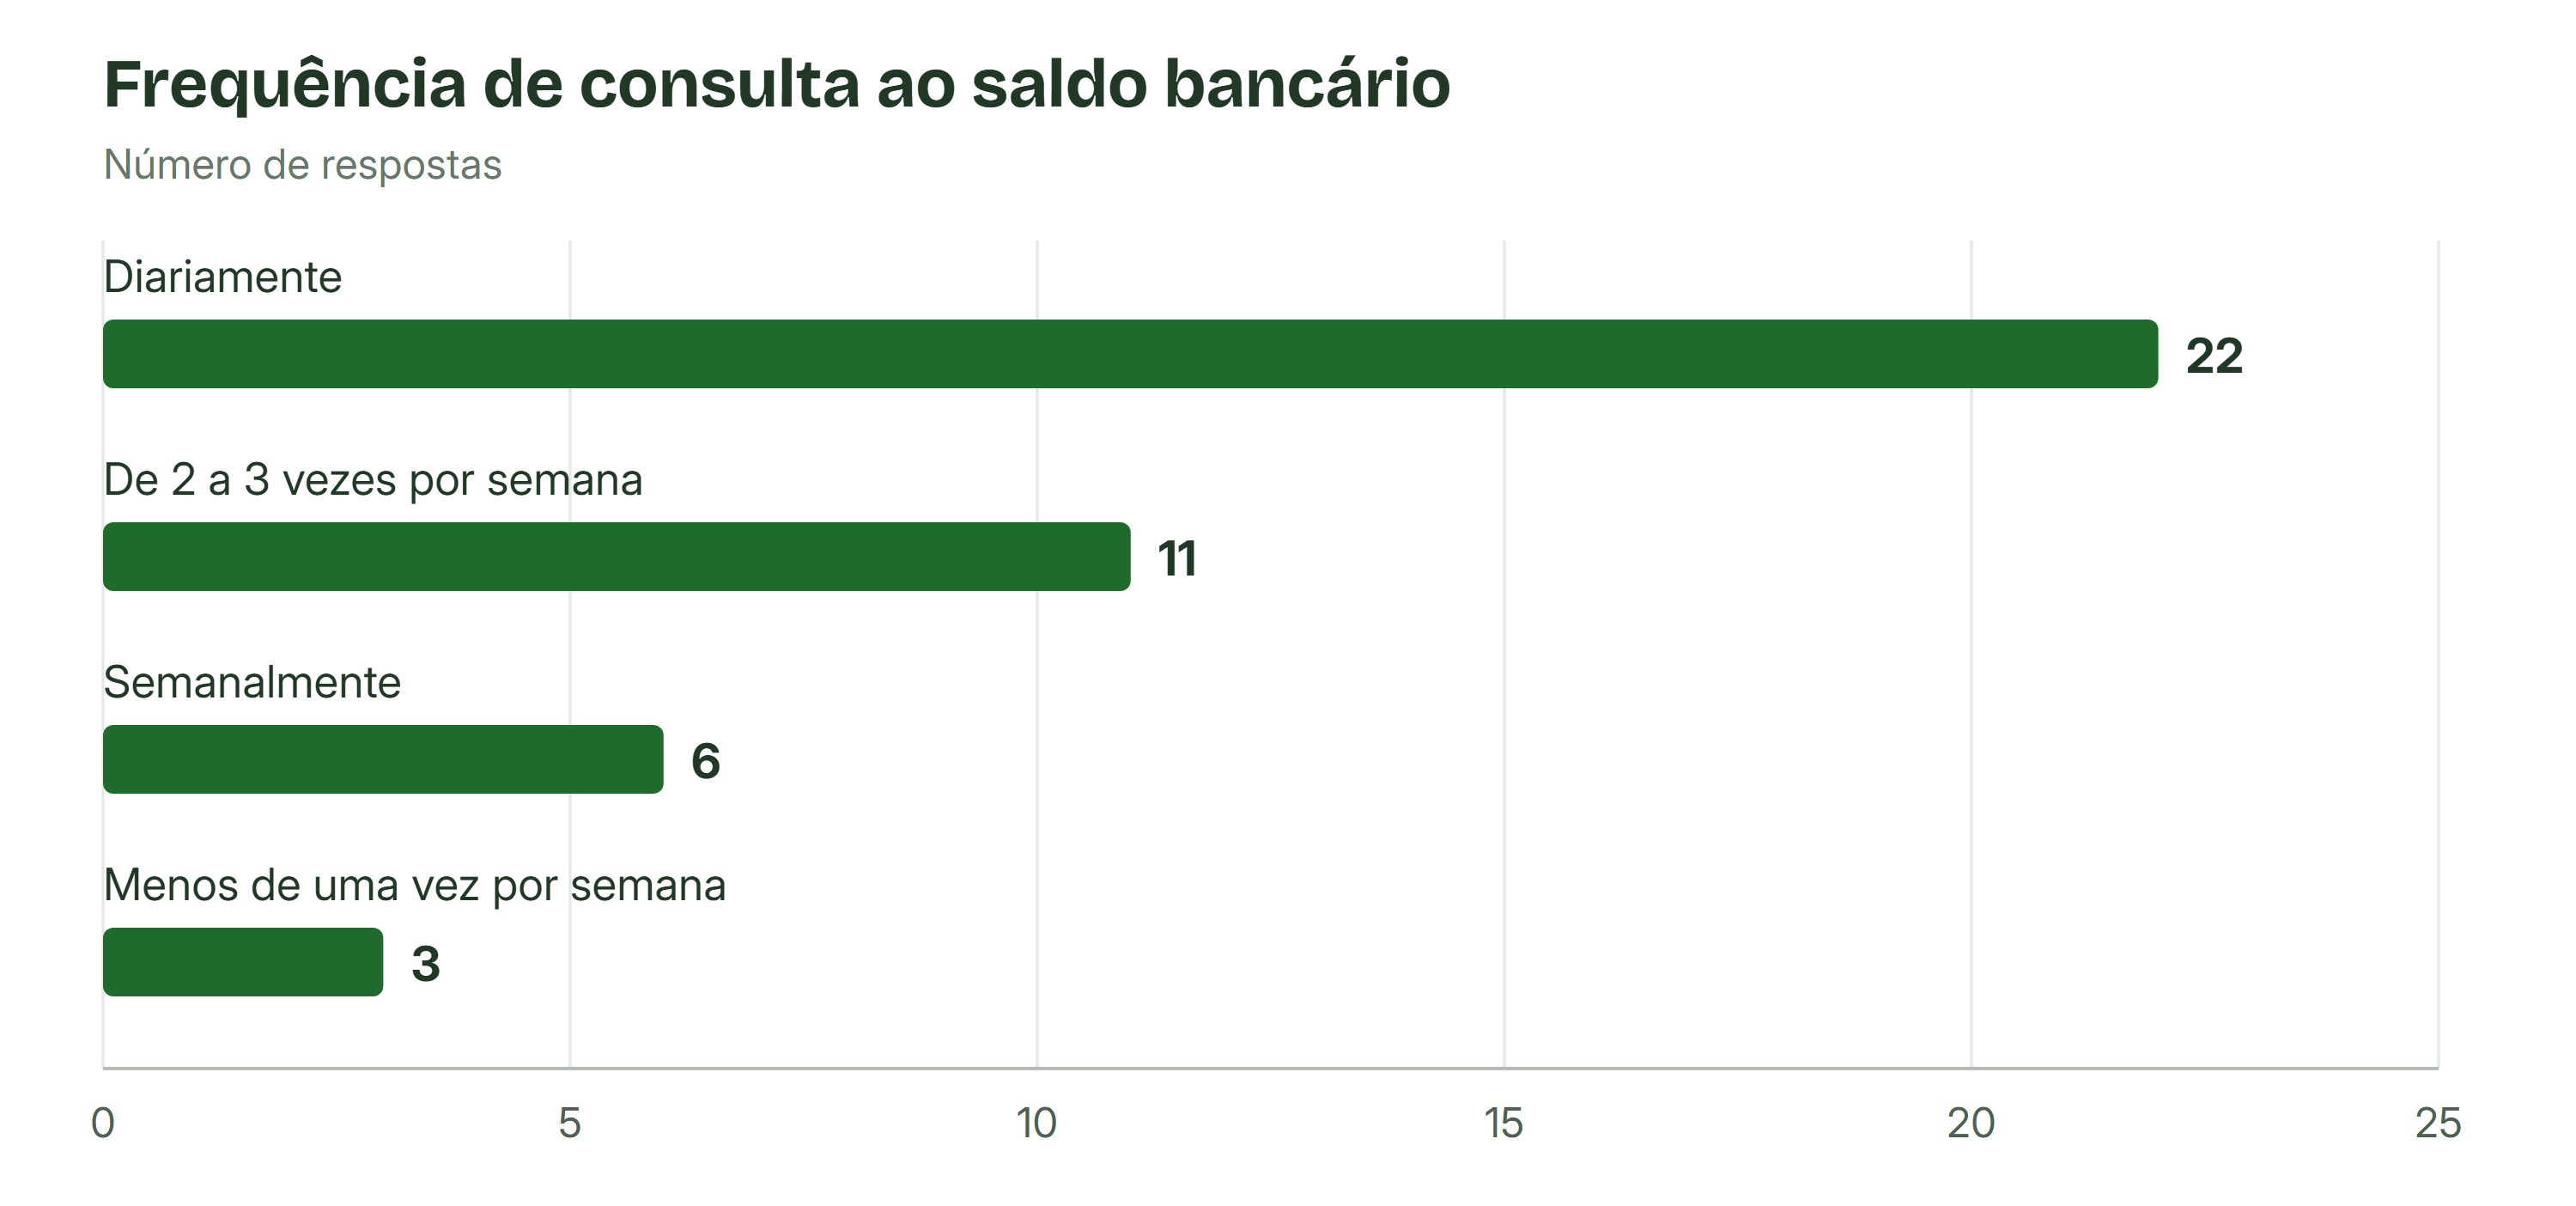
\includegraphics[width=0.8\textwidth]{images/pesquisa/frequenciaconsulta.png}
    \label{fig:pq_frequencia}
    \authorssource
\end{figure}

O gráfico da Figura \ref{fig:pq_contas} revelou que 7 participantes possuem apenas uma conta bancária ativa, enquanto 17 possuem duas contas, 12 possuem três e 6 mantêm quatro ou mais contas. Dessa forma, 35 dos 42 respondentes, correspondentes a aproximadamente 83,3\% da amostra, possuem duas ou mais contas bancárias ativas.

Esse resultado reforça a relevância de mecanismos capazes de consolidar informações financeiras distribuídas entre diferentes instituições, reduzindo a necessidade de consultas individualizadas e favorecendo uma visão mais abrangente da situação financeira do usuário. Nesse contexto, o ecossistema de \textit{Open Finance} constitui um elemento importante para viabilizar a integração dessas informações.

\begin{figure}[H]
    \centering
    \caption{Número de contas bancárias ativas dos respondentes}
    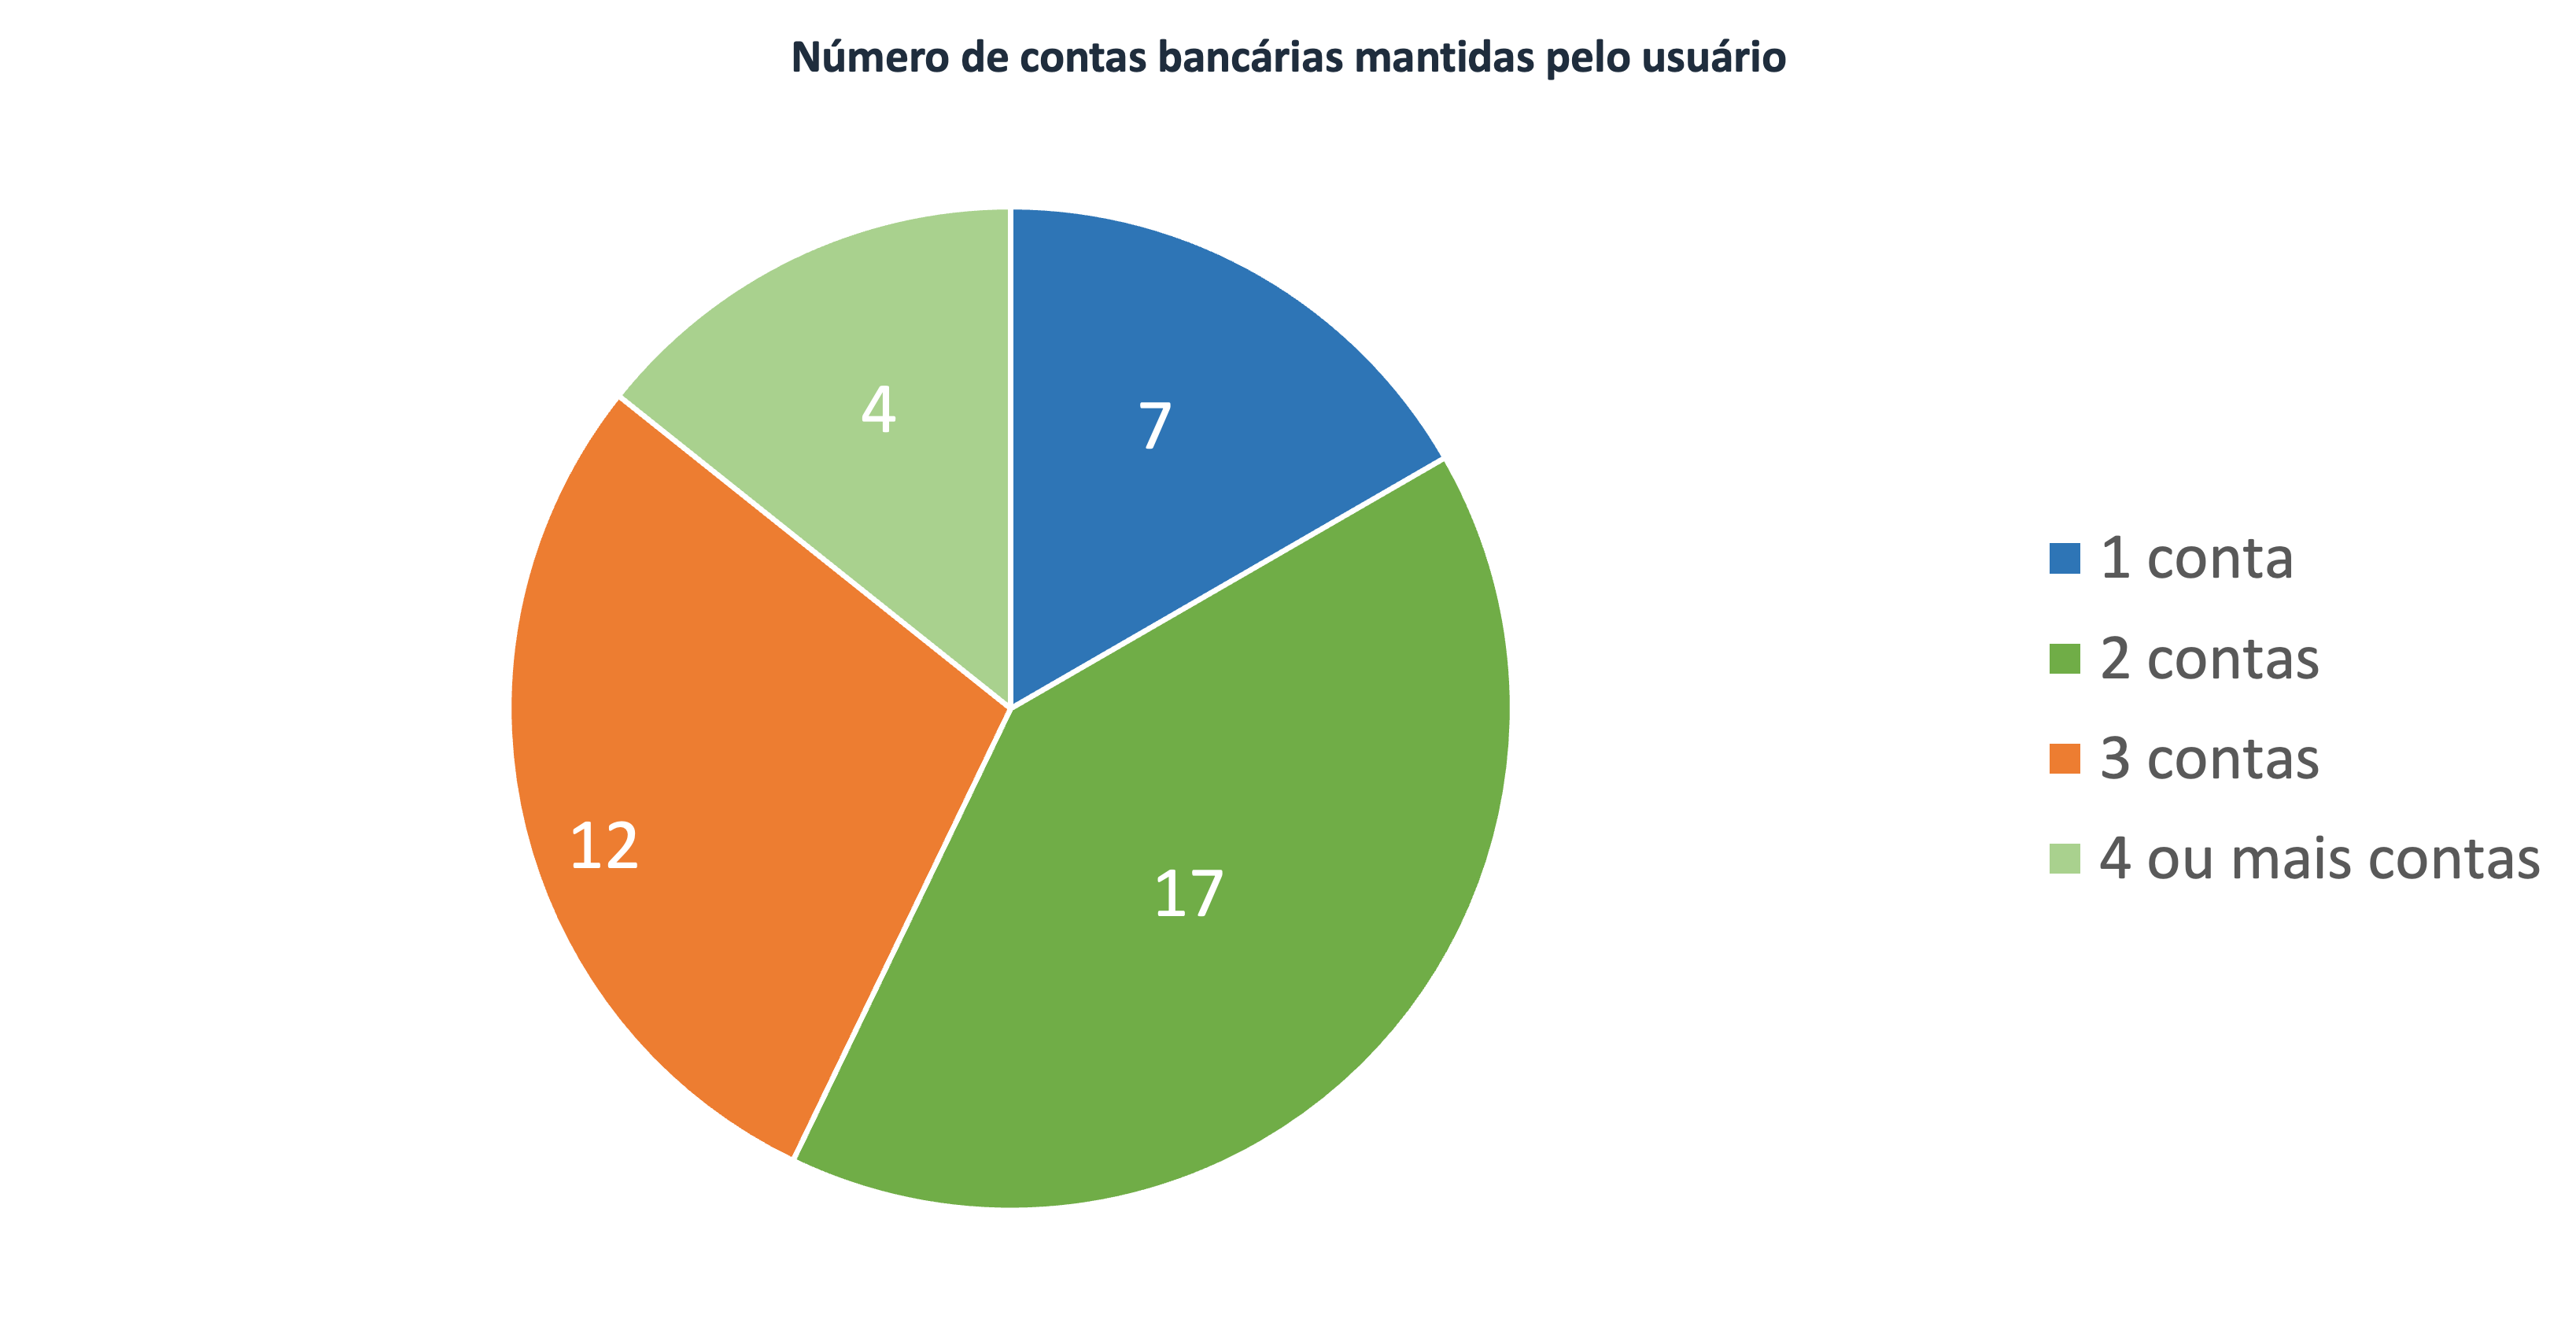
\includegraphics[width=0.8\textwidth]{images/pesquisa/numerocontas.png}
    \label{fig:pq_contas}
    \authorssource
\end{figure}

O gráfico da Figura \ref{fig:pq_openfinance} demonstrou também baixa familiaridade com o \textit{Open Finance}. Entre os participantes, 21 (50\%) declararam não conhecer o ecossistema, 17 afirmaram conhecê-lo, mas nunca o utilizaram, e apenas 4 (9,5\%) já haviam realizado o compartilhamento de dados entre instituições.

Esse resultado evidencia que, embora o \textit{Open Finance} disponibilize recursos capazes de favorecer a integração de informações financeiras, seu funcionamento e seus benefícios ainda podem não ser plenamente conhecidos por parte dos potenciais usuários. Dessa forma, a experiência oferecida pelo EIGAM também contribui para apresentar de maneira contextualizada as possibilidades proporcionadas pelo compartilhamento autorizado de dados financeiros.

\begin{figure}[H]
    \centering
    \caption{Familiaridade dos respondentes com o Open Finance}
    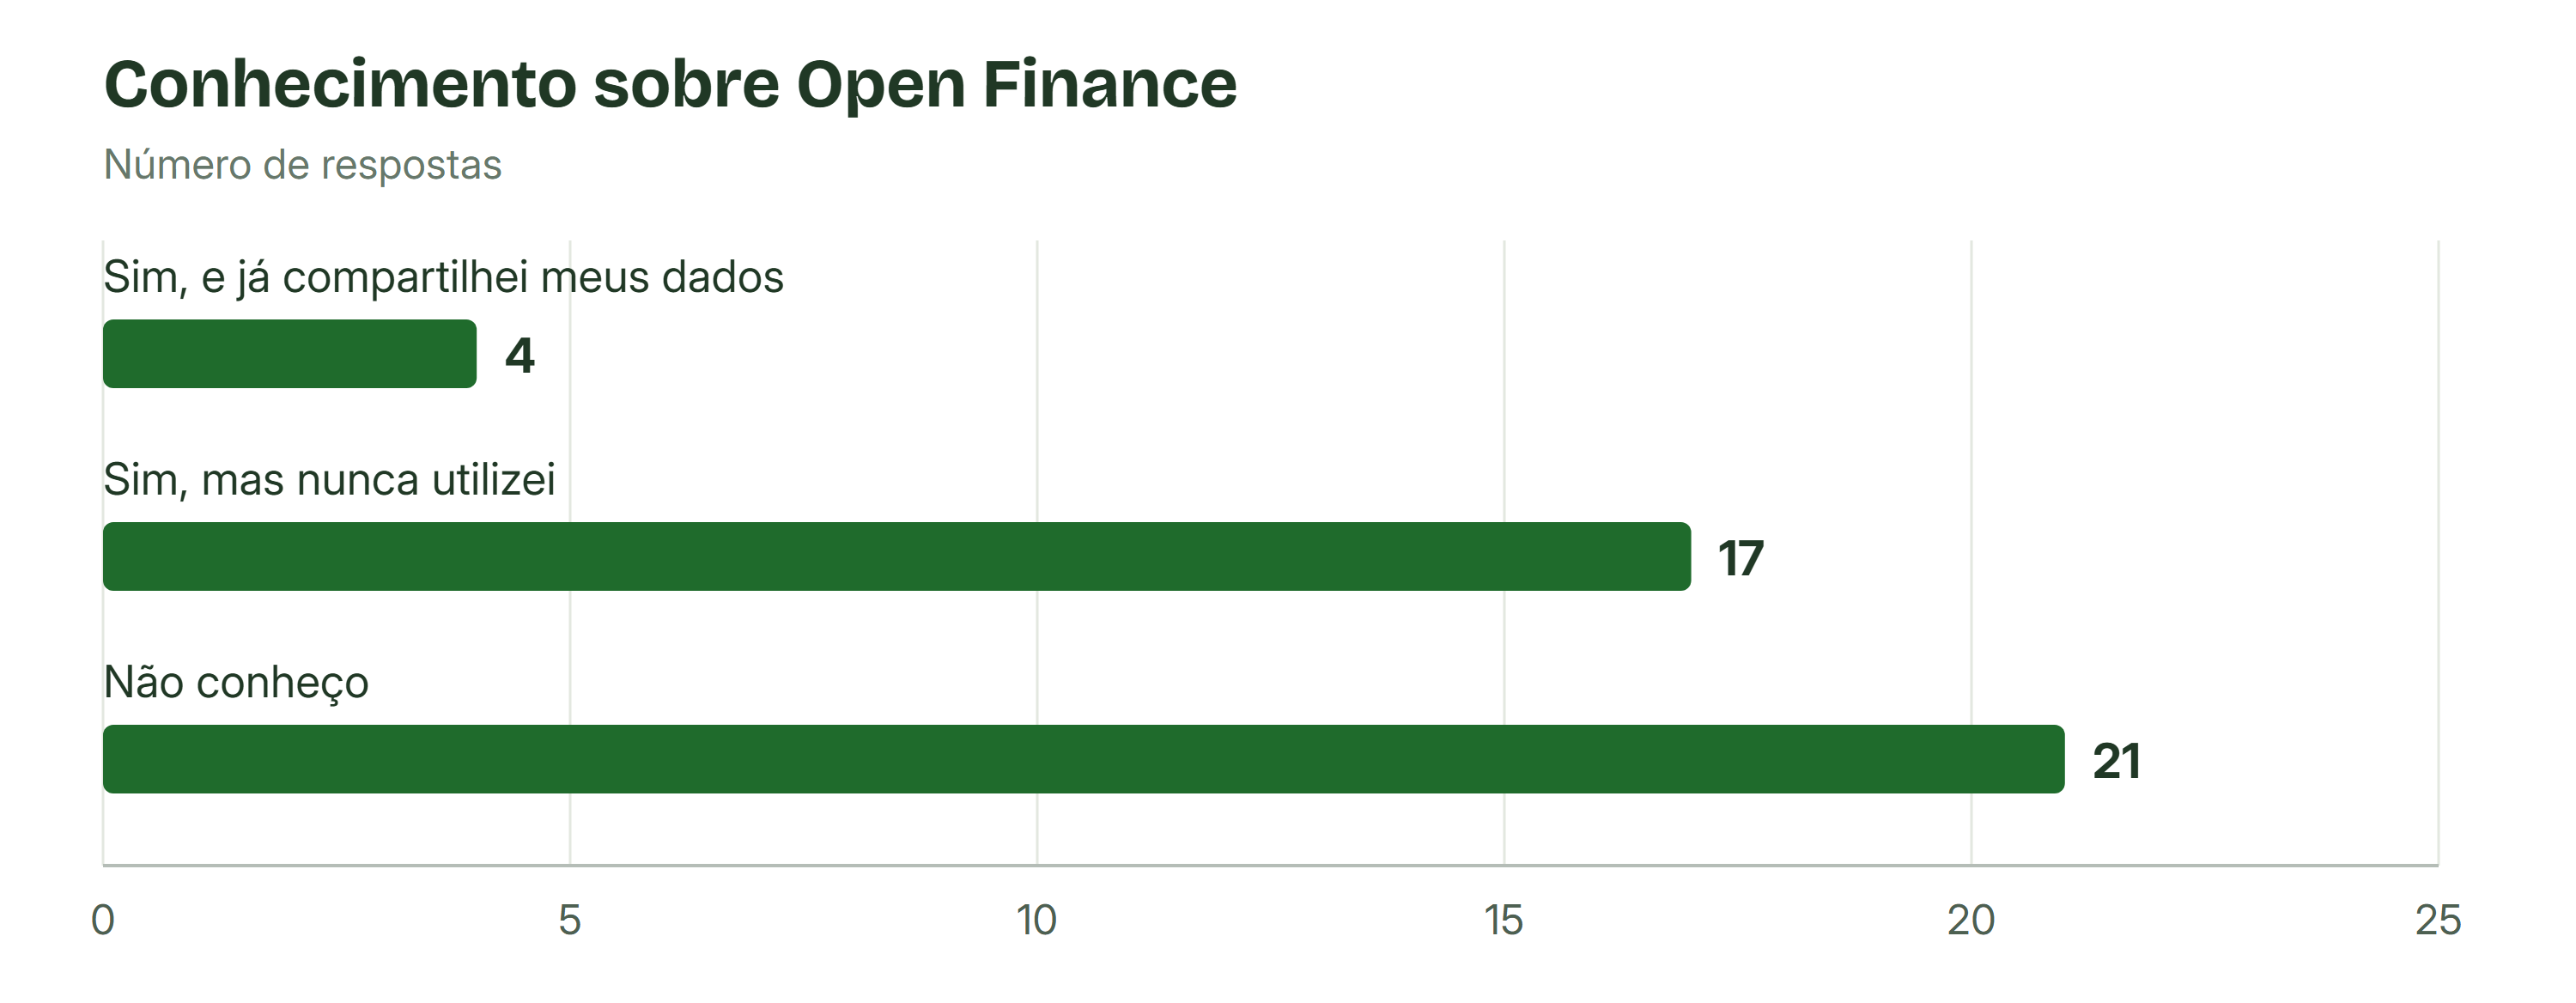
\includegraphics[width=0.8\textwidth]{images/pesquisa/conhecimentoopenfinance.png}
    \label{fig:pq_openfinance}
    \authorssource
\end{figure}

Em seguida, o gráfico da Figura \ref{fig:pq_funcionalidades} demonstrou interesse relevante pelas funcionalidades propostas. Entre as opções apresentadas, 32 participantes manifestaram interesse em resumos automáticos de gastos, 29 em alertas de vencimento de contas, 26 em previsão de saldo para os próximos dias, 23 em recomendações personalizadas e 21 em mecanismos de detecção de gastos atípicos.

A predominância de funcionalidades relacionadas à automação, previsão e geração de alertas fornece indícios de aderência à proposta de um sistema que não se limite à consulta de informações financeiras, mas que também seja capaz de analisá-las e atuar de maneira proativa no acompanhamento da vida financeira do usuário.

\begin{figure}[H]
    \centering
    \caption{Funcionalidades de maior interesse para os respondentes}
    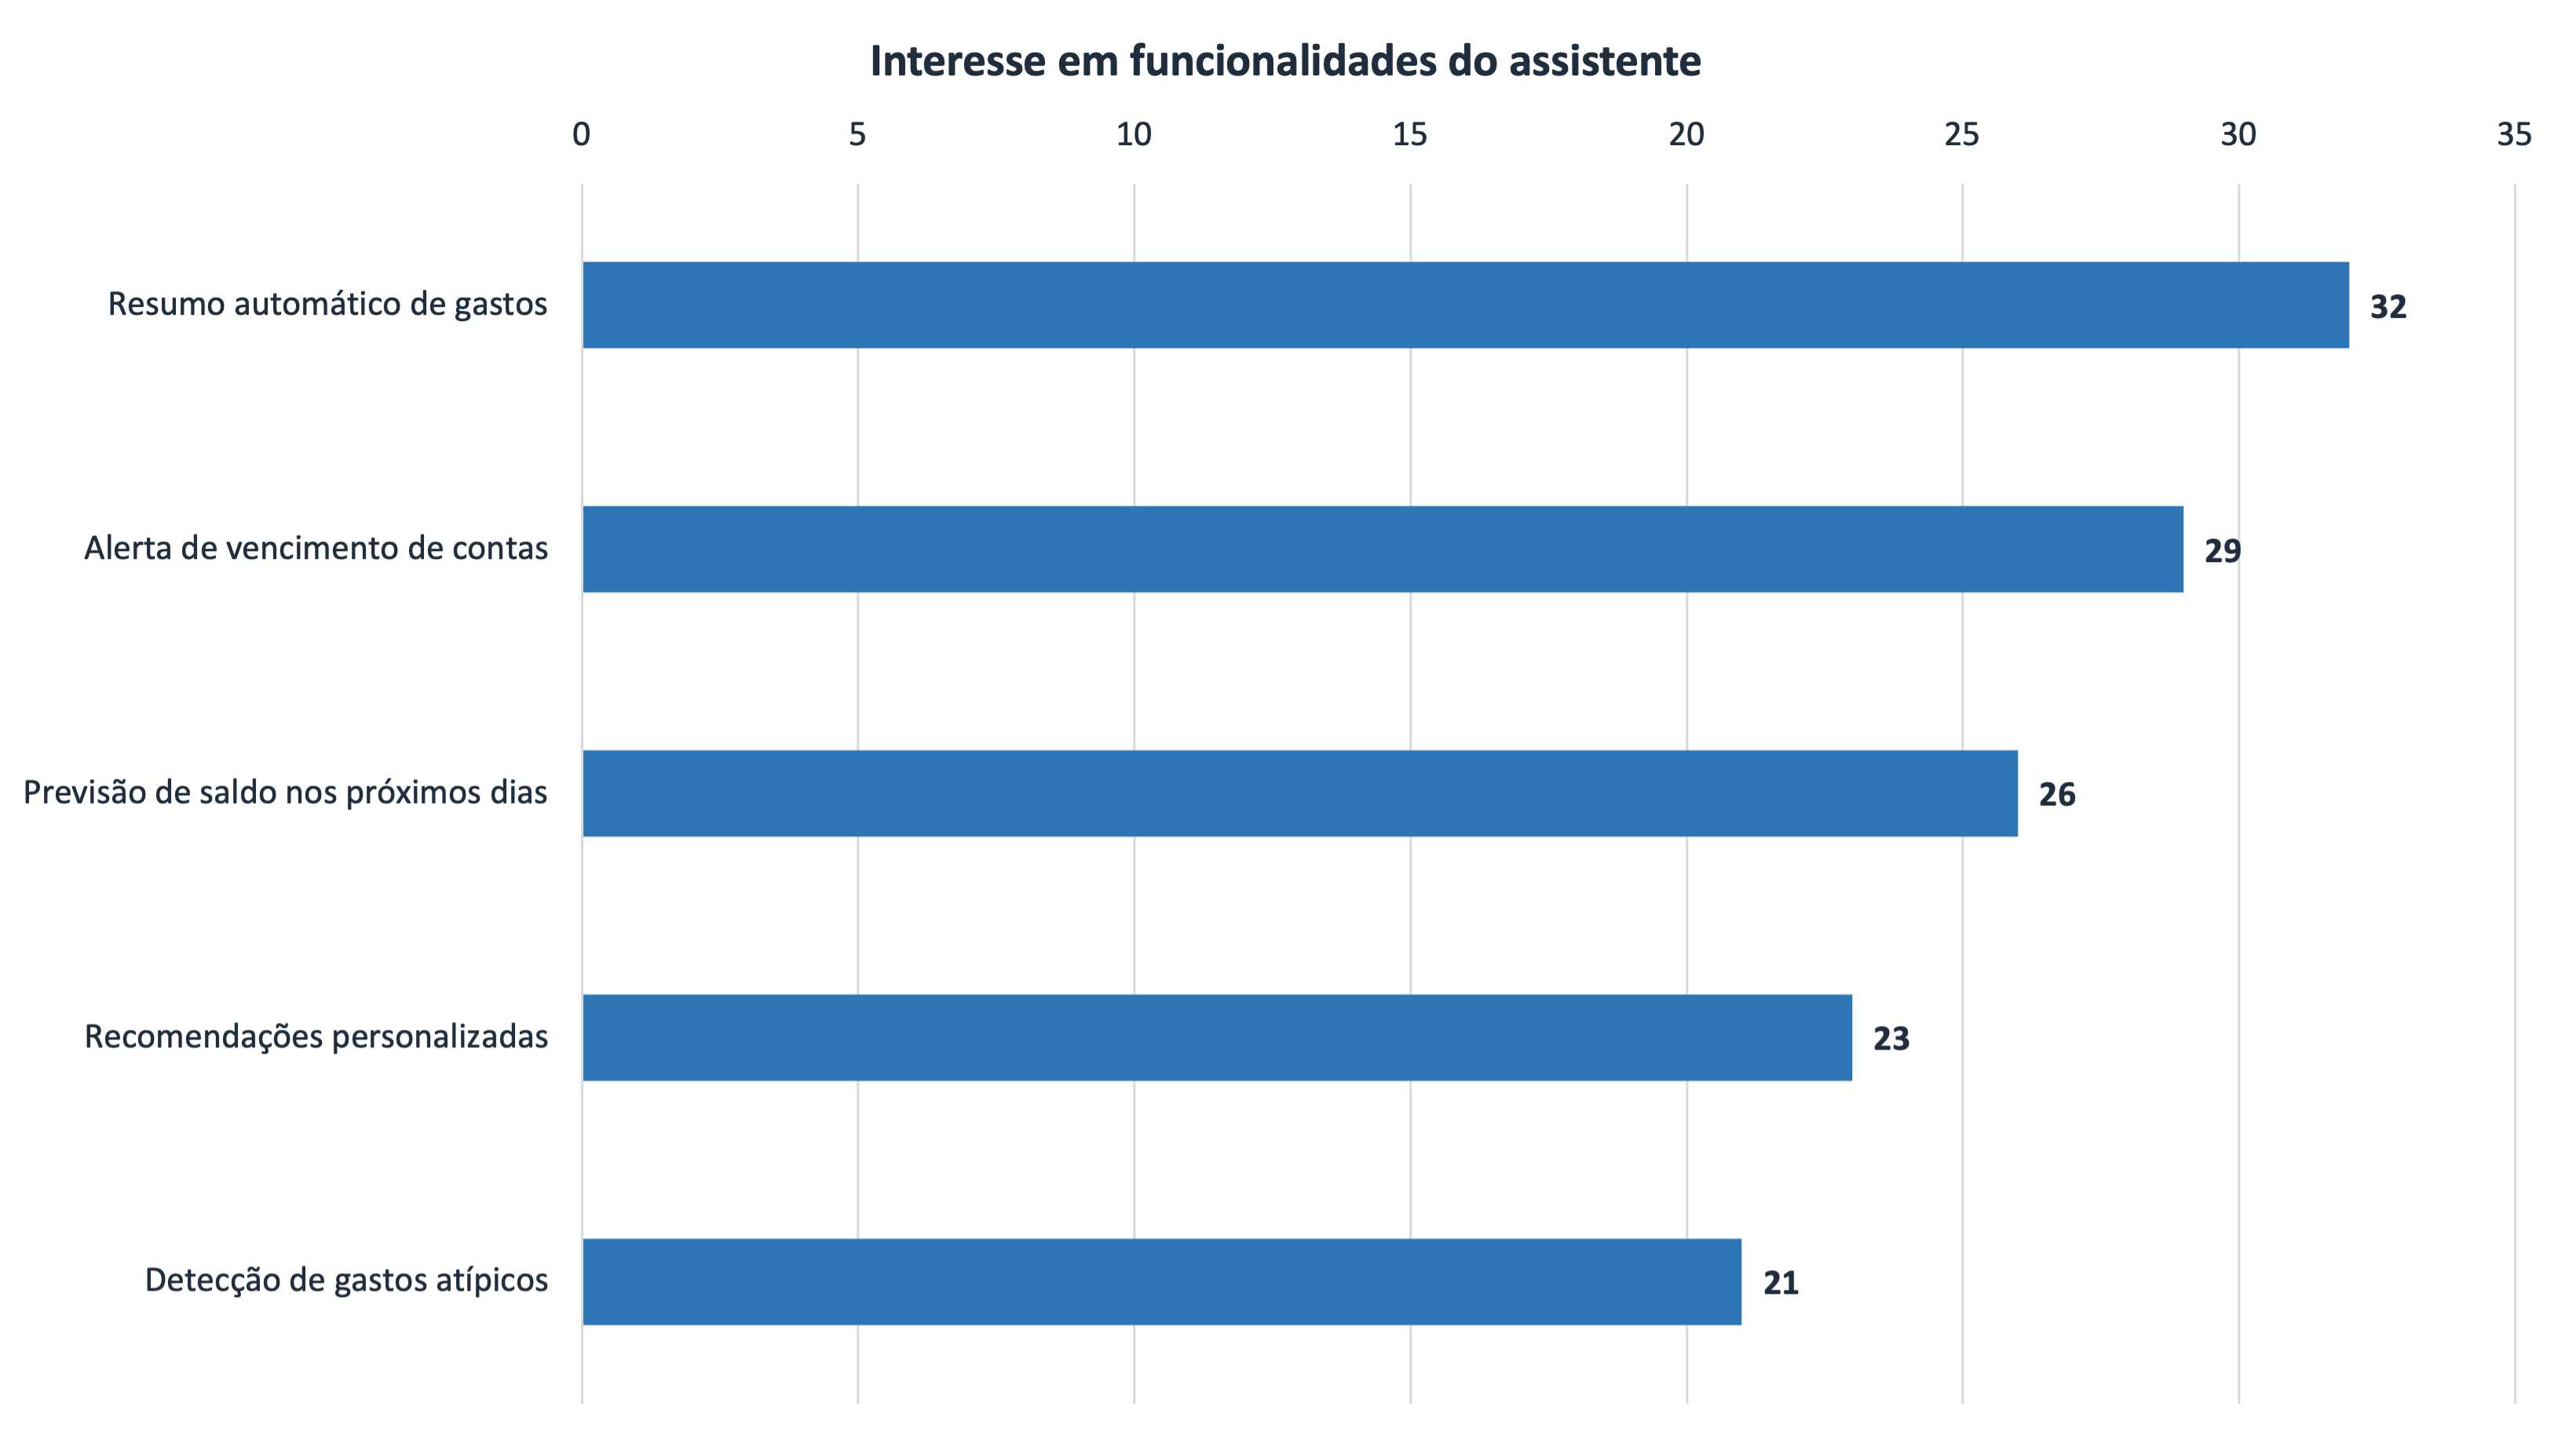
\includegraphics[width=0.8\textwidth]{images/pesquisa/interessefuncionalidade.png}
    \label{fig:pq_funcionalidades}
    \authorssource
\end{figure}

Por meio do gráfico da Figura \ref{fig:pq_confianca}, foi avaliado o nível de confiança dos participantes em um assistente conversacional baseado em inteligência artificial para tratar informações financeiras. As notas 4 e 5 somadas representam 47,6\% das respostas, correspondentes a 20 participantes, enquanto 26,2\% atribuíram notas 1 ou 2.

Os resultados demonstram que uma parcela relevante dos respondentes apresenta predisposição favorável ao uso desse tipo de tecnologia, embora também evidenciem a necessidade de mecanismos que contribuam para a construção de confiança, especialmente relacionados à transparência, à segurança e à confiabilidade das informações apresentadas.

\begin{figure}[H]
    \centering
    \caption{Nível de confiança dos respondentes em assistente conversacional com IA}
    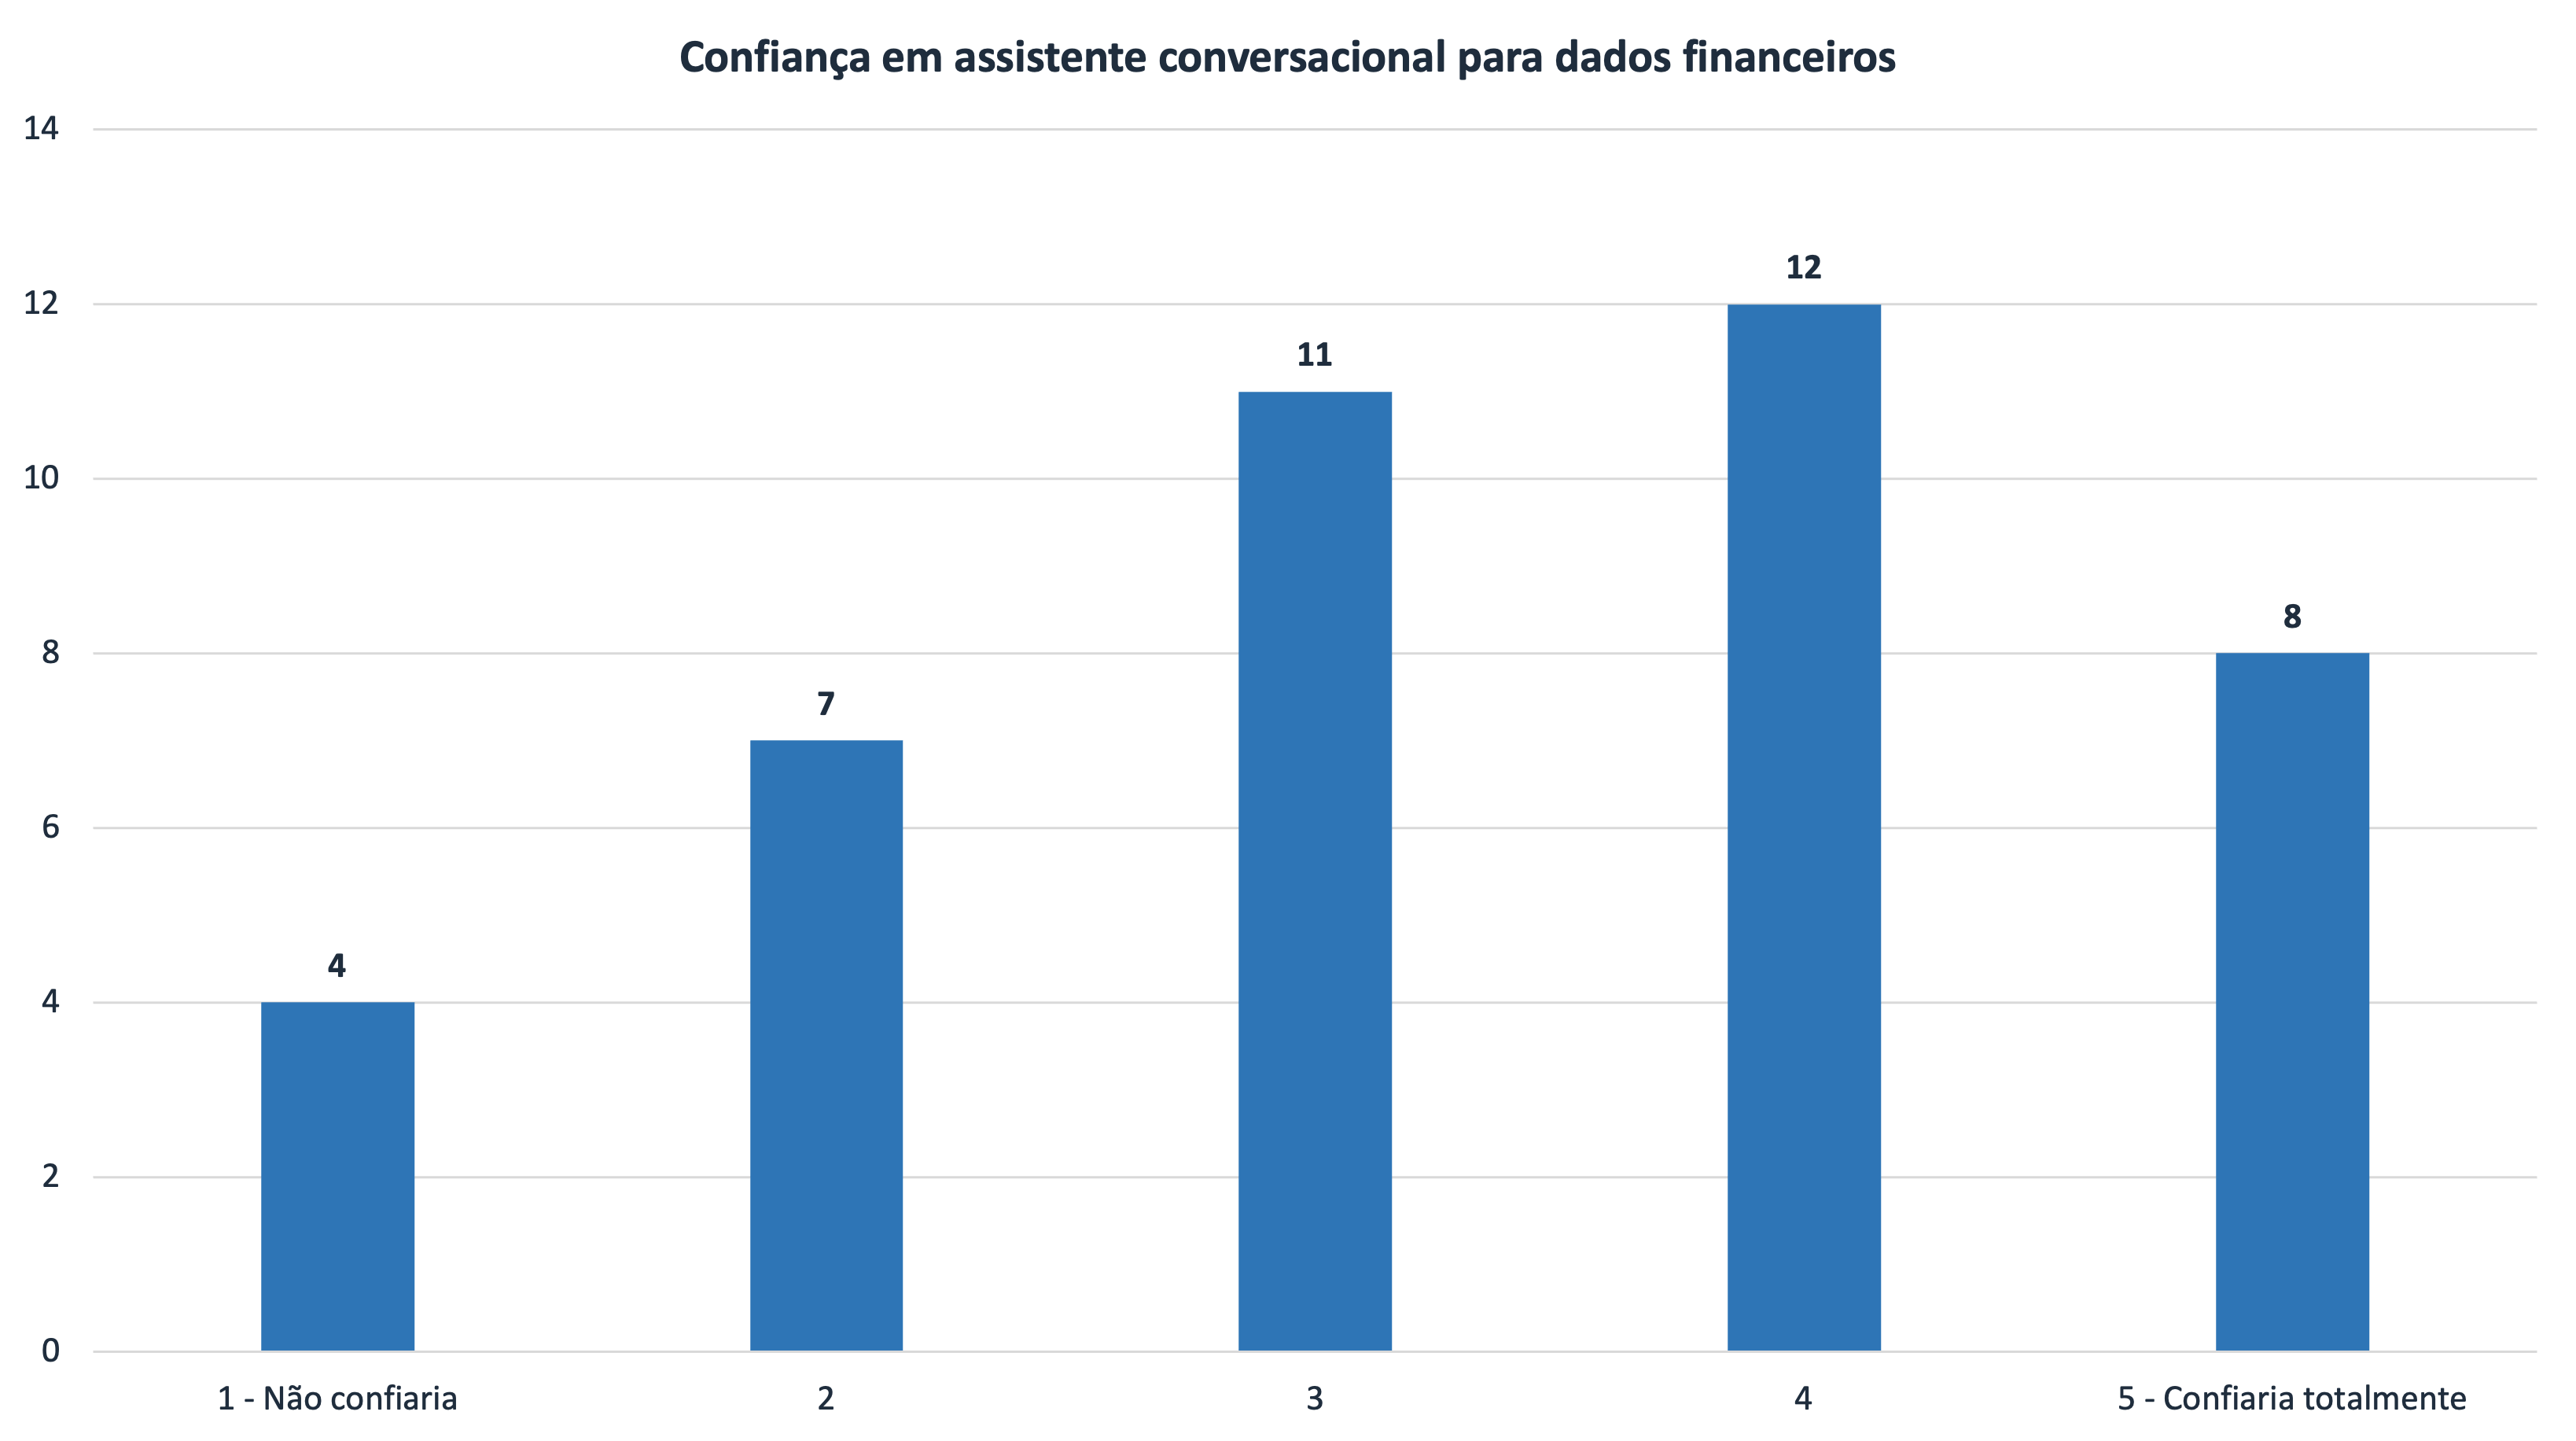
\includegraphics[width=0.8\textwidth]{images/pesquisa/confianca.png}
    \label{fig:pq_confianca}
    \authorssource
\end{figure}

O gráfico da Figura \ref{fig:pq_privacidade} indicou elevado nível de preocupação com a privacidade dos dados financeiros. Entre os respondentes, 15 (35,7\%) atribuíram nota máxima e 14 (33,3\%) atribuíram nota 4, totalizando aproximadamente 69\% dos participantes com nível elevado de preocupação.

Esse resultado reforçou a necessidade de que o EIGAM incorporasse mecanismos de autenticação, controle de acesso, proteção dos dados e gerenciamento de consentimentos, além de apresentar ao usuário de maneira transparente como suas informações financeiras são utilizadas.

\begin{figure}[H]
    \centering
    \caption{Nível de preocupação dos respondentes com a privacidade de dados financeiros}
    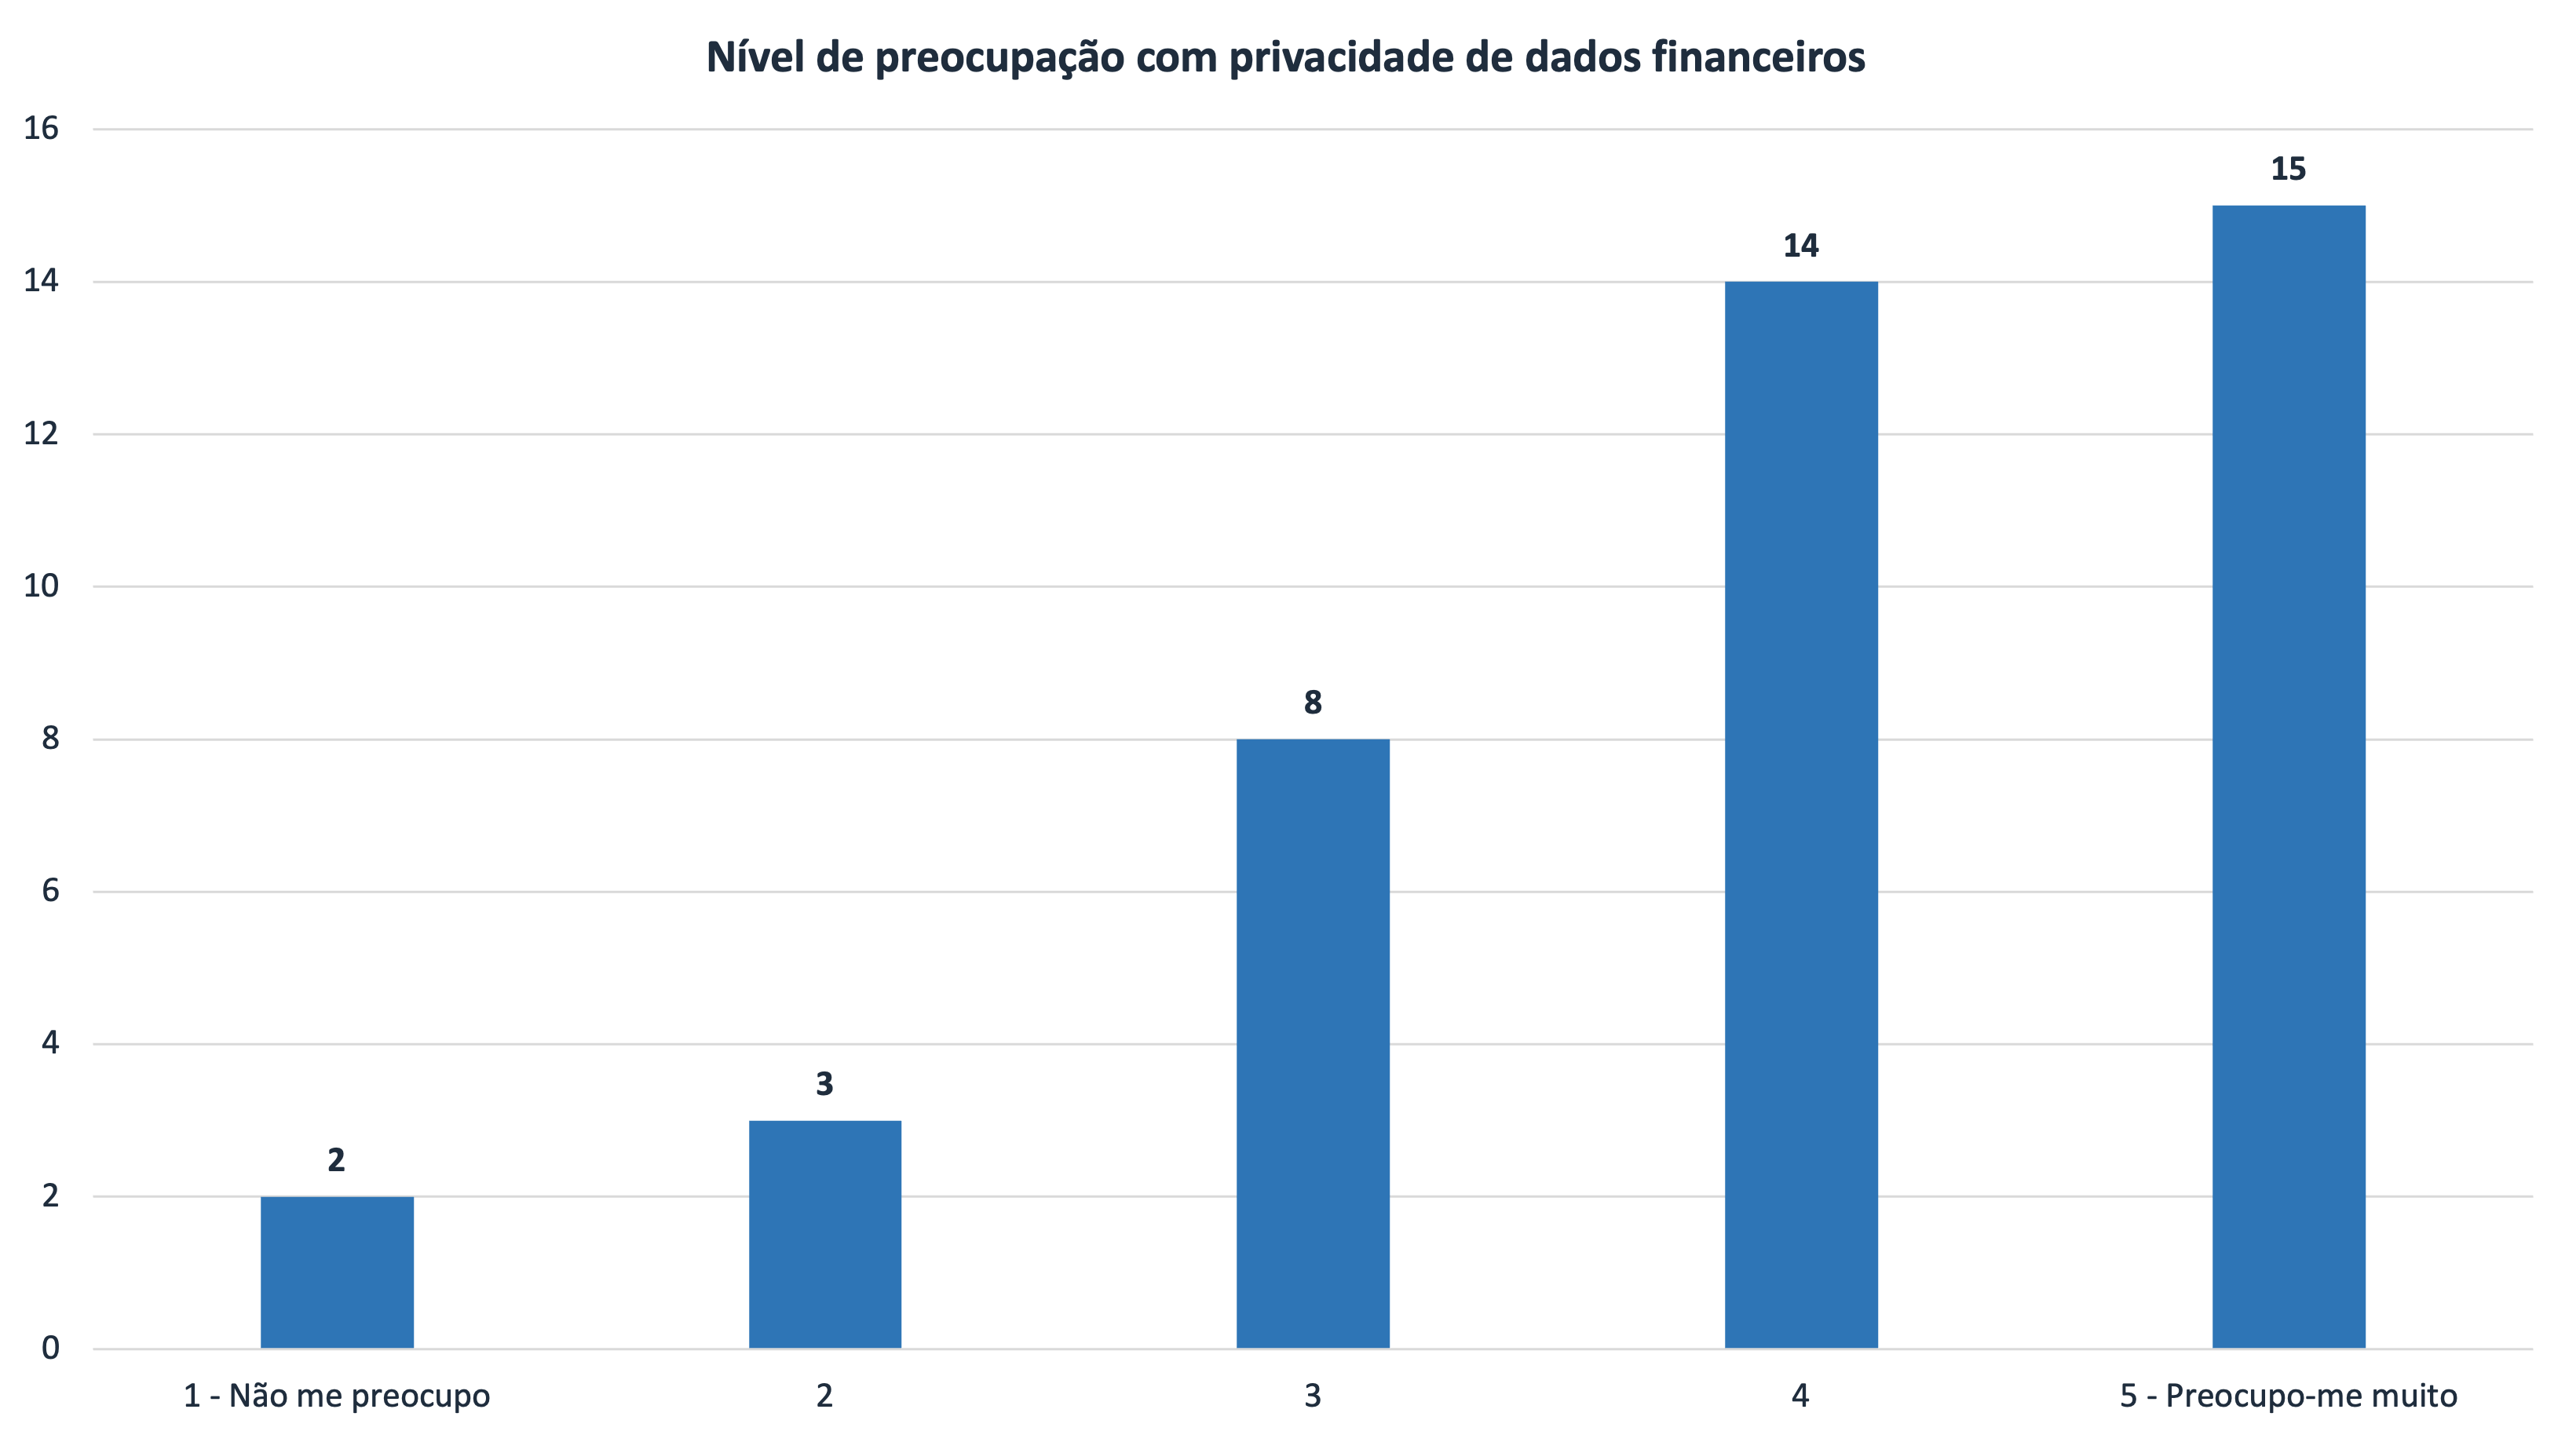
\includegraphics[width=0.8\textwidth]{images/pesquisa/nivelpreocupacao.png}
    \label{fig:pq_privacidade}
    \authorssource
\end{figure}

Finalmente, o gráfico da Figura \ref{fig:pq_pagamento} avaliou a disposição dos participantes em pagar por um plano premium. Apenas 7 respondentes (16,7\%) afirmaram que não pagariam pelo serviço, enquanto 12 (28,6\%) indicaram disposição de pagar até R\$~10,00, 15 (35,7\%) entre R\$~11,00 e R\$~20,00, 6 (14,3\%) entre R\$~21,00 e R\$~30,00 e 2 (4,8\%) acima de R\$~30,00 mensais.

Os resultados indicam a existência de disposição de pagamento em parcela relevante da amostra, embora também demonstrem sensibilidade ao preço. Dessa forma, os dados obtidos não são utilizados isoladamente para determinar o valor comercial do produto, mas constituem uma das referências consideradas na definição do modelo de monetização apresentado na Seção \ref{sec:preco}.

\begin{figure}[H]
    \centering
    \caption{Disposição dos respondentes para pagar por plano premium}
    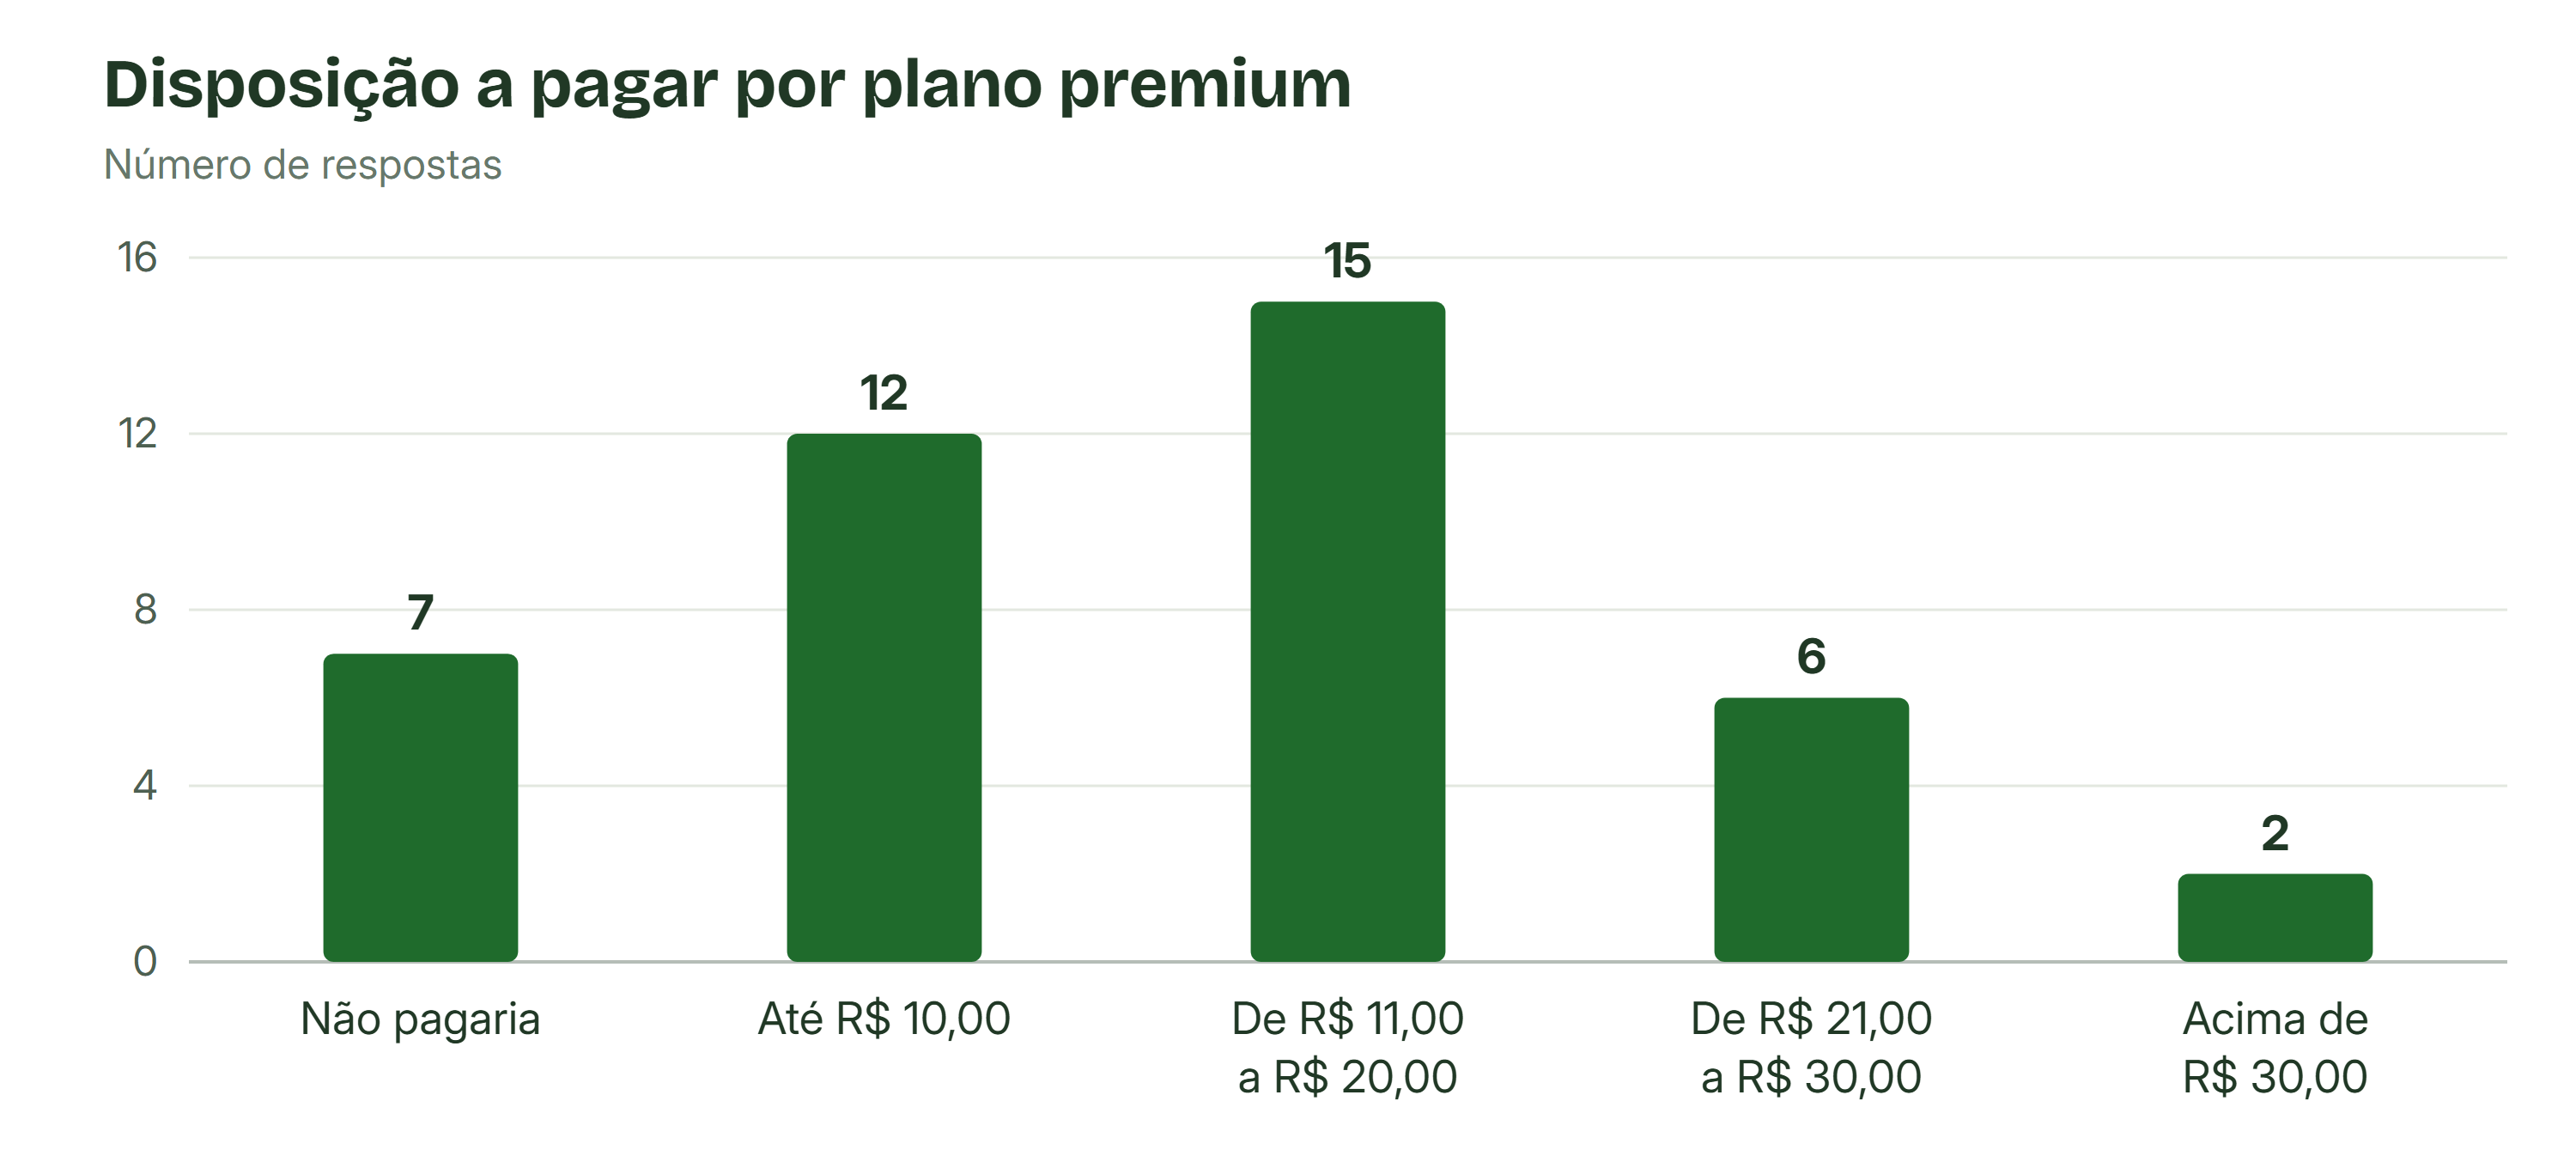
\includegraphics[width=0.8\textwidth]{images/pesquisa/pagarplano.png}
    \label{fig:pq_pagamento}
    \authorssource
\end{figure}

De maneira geral, os resultados obtidos fornecem indícios favoráveis à proposta apresentada. A elevada presença de participantes com múltiplas contas bancárias reforça o problema de fragmentação das informações financeiras; o interesse por resumos, previsões e alertas demonstra aderência às funcionalidades preditivas e proativas propostas; e a ampla utilização do \textit{WhatsApp} na amostra sustenta sua escolha como canal inicial de interação.

Ao mesmo tempo, os resultados relacionados à confiança e à privacidade evidenciaram aspectos que receberam atenção especial na construção e na validação da solução. Ressalta-se que, devido ao tamanho e às características da amostra utilizada, os resultados obtidos representam indícios relacionados ao grupo pesquisado e não devem ser interpretados como uma generalização do comportamento de toda a população.

\section{Análise da concorrência}

A análise da concorrência considerou três soluções brasileiras que também utilizam inteligência artificial no acompanhamento das finanças pessoais e que, como o EIGAM, se apoiam na conversa ou no \textit{Open Finance}: o Pierre, assistente financeiro da CloudWalk; o Jota, assistente e conta digital que funciona dentro do \textit{WhatsApp}; e o Visor, aplicativo de finanças pessoais com assistente de IA. O Quadro~\ref{frame:concorrencia} compara as quatro soluções a partir das informações públicas dos próprios produtos e de reportagens sobre eles.

{\footnotesize
\begin{longtable}{|L{2.6cm}|L{3.25cm}|L{3.05cm}|L{3.05cm}|L{3.05cm}|}
\caption{Comparação do EIGAM com soluções concorrentes}
\label{frame:concorrencia} \\
\continuesmark

\hline
\textbf{Critério} & \textbf{EIGAM} & \textbf{Pierre} & \textbf{Jota} & \textbf{Visor} \\ \hline
\endfirsthead

\hline
\textbf{Critério} & \textbf{EIGAM} & \textbf{Pierre} & \textbf{Jota} & \textbf{Visor} \\ \hline
\endhead

\endfoot
\multicolumn{5}{p{15.6cm}}{\rule{0pt}{\dimexpr 0.3cm+2ex\relax}\centering\fontsize{10pt}{12pt}\selectfont\textbf{Fonte:} Elaborado pelos autores (\workYear), com base em Pierre (2026), Lopes (2026), Rios (2025), Paiva (2025), Com Celcoin [...] (2026), Visor (2026), Magro (2026) e Visor integra [...] (2026). ``Não informado'' indica que a informação não consta nas fontes consultadas.} \\
\endlastfoot

Canal de uso &
Conversa no \textit{WhatsApp} e no \textit{Telegram}, painel \textit{web} e assistentes de IA do titular &
Aplicativo para iOS e Android &
Conversa no \textit{WhatsApp} &
Aplicativo, \textit{web} e \textit{WhatsApp} \\ \hline

\textit{Open Finance} &
Sim, somente leitura: contas, cartões, investimentos e empréstimos &
Sim &
Não informado &
Sim, somente leitura \\ \hline

Pagamentos &
Não realiza &
Agente que navega na internet para fazer compras (Pierre Computer) &
Conta digital própria, com Pix e boletos por texto, áudio ou imagem &
Pix pelo chat, confirmado por biometria \\ \hline

Planejamento e previsões &
Projeção do gasto do mês em faixa, saldo livre do fim do mês, simulação de compra, metas e resumos periódicos &
Não informado &
Não informado &
Projeção de saldo, quanto ainda dá para gastar no mês, simulação de compra e limites por categoria \\ \hline

Acesso por assistentes de IA externos &
Sim, por servidor MCP, no plano Pro &
Sim, pelo protocolo Pierre MCP &
Não informado &
Sim, pelo ChatGPT e pelo Claude (MCP), nos planos pagos \\ \hline

Proteção dos valores &
Valores ocultos na conversa e no painel até a confirmação do PIN de seis dígitos &
Não informado &
Não informado &
Biometria para confirmar o Pix \\ \hline

Público principal &
Jovens de 18 a 30 anos &
Pessoas físicas &
Microempreendedores e pequenas empresas, além de pessoas físicas &
Pessoas físicas \\ \hline

Modelo de cobrança &
Teste de 7 dias; Pro a R\$~29,90/mês ou R\$~328,90/ano &
Básico gratuito; Pro a R\$~39/mês, com até cinco bancos; Premium a R\$~199/mês &
Gratuito, com cobrança prevista por operação &
Teste grátis; planos Basic (1 banco), Pro (até 3) e Premium (sem limite), de R\$~239,90 a R\$~699,00 por ano \\ \hline

\end{longtable}
}

A comparação mostra que as soluções partem do mesmo ponto do EIGAM: dados reunidos pelo \textit{Open Finance} e consulta em linguagem natural. As diferenças estão no canal, no escopo e no modelo de cobrança. O Pierre e o Visor partem de um aplicativo próprio, e o Jota une a conversa no \textit{WhatsApp} a uma conta de pagamentos voltada principalmente a pequenos empreendedores. O EIGAM se diferencia por funcionar dentro das ferramentas de conversa que o usuário já utiliza, inclusive no assistente de IA do próprio titular, por apresentar as estimativas em faixa e se abster quando não há confiança estatística, e por tornar a privacidade visível, com os valores ocultos até a confirmação do PIN. O plano Pro do EIGAM também custa menos que o Pro do Pierre e que o Pro anual do Visor.

Em contrapartida, o EIGAM não movimenta dinheiro, enquanto o Jota e o Visor já permitem pagamentos pela conversa e o Pierre avança para agentes que executam compras. A ausência de pagamentos reduz a exposição regulatória e o risco de uma transação indevida, mas representa uma lacuna diante desses concorrentes, que contam ainda com bases de usuários e marcas já estabelecidas. Esse cenário reforça a ameaça de concorrência registrada na Matriz SWOT (Figura~\ref{fig:swot}) e orienta o preço apresentado na Seção~\ref{sec:preco}.

\section{Análise de viabilidade}

A viabilidade do projeto foi analisada sob três perspectivas complementares: técnico-operacional, econômica e regulatória. A perspectiva técnico-operacional considera os recursos necessários à implementação, integração e manutenção da solução; a perspectiva econômica considera os custos associados à infraestrutura e aos serviços externos em diferentes estágios de utilização; e a perspectiva regulatória considera aspectos relacionados ao tratamento de dados pessoais e financeiros e à utilização de serviços externos.

\subsection{Viabilidade Operacional e Econômica}

A infraestrutura é composta por um único servidor virtual em um provedor de nuvem, descrito em Terraform, no qual o \textit{broker}, o Redis, o PostgreSQL, a observabilidade e os quatorze serviços da aplicação são executados em contêineres. Essa composição oferece custo previsível e permite reconstruir o ambiente inteiro a partir do repositório. No caso do \textit{broker}, o menor plano pago de um serviço gerenciado superaria o orçamento mensal de toda a infraestrutura do projeto.

O \textit{WhatsApp} é o principal canal de mensageria, e o \textit{Telegram} não acrescenta custo de infraestrutura, pois utiliza o mesmo \textit{gateway} e o mesmo \textit{worker} de envio. A arquitetura multicanal, portanto, representou uma decisão de organização do software, e não a contratação simultânea de diferentes serviços.

O Quadro~\ref{frame:infra_dev} apresenta os recursos efetivamente utilizados no desenvolvimento e na operação do beta. Os custos fixos estão em euros, moeda de cobrança do provedor de nuvem; os custos variáveis são os preços unitários registrados na tabela de preços do próprio sistema, utilizada para calcular o custo de cada titular.

{\small
\begin{longtable}{|L{3.3cm}|L{7.2cm}|L{3.5cm}|}
\caption{Infraestrutura e serviços utilizados no desenvolvimento e no beta}
\label{frame:infra_dev} \\
\continuesmark

\hline
\textbf{Componente} & \textbf{Especificação} & \textbf{Custo} \\ \hline
\endfirsthead

\hline
\textbf{Componente} & \textbf{Especificação} & \textbf{Custo} \\ \hline
\endhead

\endfoot
\sourcerow{3} \\
\endlastfoot

Servidor &
Hetzner CX33 (4 vCPU, 8 GB de RAM, 80 GB de SSD), executando todos os serviços por meio de Docker Compose &
$\sim$€~9,99/mês \\ \hline

Volume cifrado &
40 GB com LUKS para os dados do PostgreSQL, preservado mesmo quando o servidor é recriado &
$\sim$€~2/mês \\ \hline

\textit{Broker}, cache e banco relacional &
Redpanda, Redis e PostgreSQL 16 com pgvector, executados no próprio servidor &
Incluído no servidor \\ \hline

Banco documental &
MongoDB Atlas M0 &
Plano gratuito \\ \hline

Observabilidade &
Prometheus, Loki, Tempo, Grafana e Alertmanager, executados no próprio servidor &
Incluído no servidor \\ \hline

Borda e certificados &
Cloudflare (\textit{proxy}, DNS, túnel e Access) e Let's Encrypt &
Plano gratuito \\ \hline

Modelo de linguagem &
OpenAI, no planejamento da frase e na redação da resposta &
R\$~0,016 a R\$~0,019 por chamada ao planejador \\ \hline

Juízo tipado &
TypeSafe, nos \textit{guardrails} de conselho regulado e de \textit{prompt injection} &
US\$~0,042 por milhão de \textit{tokens} \\ \hline

Mensageria &
\textit{WhatsApp}: mensagem de serviço ou utilidade (acima de 1.000 gratuitas por mês) e mensagem de marketing; \textit{Telegram} sem cobrança &
R\$~0,035 e R\$~0,3217 por mensagem \\ \hline

Integração \textit{Open Finance} &
Pluggy, por conexão bancária ativa no mês (até 500 conexões; R\$~2,50 acima disso) &
R\$~5,00 por conexão \\ \hline

Pagamentos &
Stripe, por cobrança de cartão &
3,99\% + R\$~0,39 \\ \hline

Equipamentos (depreciação) &
3 notebooks para desenvolvimento, considerando vida útil de 4 anos e valor médio de R\$~5.000 por equipamento &
$\sim$R\$~312/mês \\ \hline

IA para apoio ao desenvolvimento &
Ferramentas de inteligência artificial utilizadas pela equipe como apoio à programação &
$\sim$R\$~330/mês \\ \hline

\end{longtable}
}

O custo fixo medido da infraestrutura foi de cerca de 12 euros mensais, para quatorze serviços, três bancos de dados, o \textit{broker} e a observabilidade completa. A maior parte do custo da equipe continua sendo a depreciação dos equipamentos e as ferramentas de apoio ao desenvolvimento, que não representam custo de manter a aplicação disponível.

Com a aplicação em funcionamento, o teste de carga descrito no Capítulo~\ref{chap:resultados} mostrou que o mesmo servidor atende cerca de 2.850 usuários com boa experiência, e que o limite não é o processamento, mas o tempo de espera pelo modelo de linguagem. Para uma operação de produção, a topologia planejada separa aplicação, dados e \textit{broker} em três servidores na mesma rede privada, com balanceador de carga, armazenamento de objetos para \textit{backups} e um plano pago do MongoDB Atlas, como apresenta o Quadro~\ref{frame:infra_prod}.

{\small
\begin{longtable}{|L{3.5cm}|L{7.0cm}|L{3.0cm}|}
\caption{Infraestrutura planejada para a operação de produção}
\label{frame:infra_prod} \\
\continuesmark

\hline
\textbf{Componente} & \textbf{Especificação} & \textbf{Custo/mês} \\ \hline
\endfirsthead

\hline
\textbf{Componente} & \textbf{Especificação} & \textbf{Custo/mês} \\ \hline
\endhead

\endfoot
\sourcerow{3} \\
\endlastfoot

Servidor de aplicação &
Hetzner CX32 (4 vCPU, 8 GB de RAM) com os serviços e o Nginx &
$\sim$€~14 \\ \hline

Servidor de dados &
Hetzner CX32 com PostgreSQL e Redis, sem IP público &
$\sim$€~14 \\ \hline

Servidor do \textit{broker} &
Hetzner CX22 (2 vCPU, 4 GB de RAM) com o Redpanda, sem IP público &
$\sim$€~5 \\ \hline

Balanceador e volume &
Balanceador LB11 e volume de 100 GB cifrado com LUKS &
$\sim$€~11 \\ \hline

Armazenamento de objetos &
\textit{Backups} cifrados &
$\sim$€~6 \\ \hline

Banco documental &
MongoDB Atlas M10 &
$\sim$€~52 \\ \hline

\textbf{Custo-base estimado} &
\textbf{Não inclui modelo de linguagem, mensageria, \textit{Open Finance} e pagamentos} &
\textbf{$\sim$€~100} \\ \hline

\end{longtable}
}

A partir dessa composição, o custo mensal da operação deve ser entendido como a soma de um custo-base de infraestrutura, pequeno e previsível, com custos variáveis que crescem com cada titular. A medição feita pelo próprio sistema mostrou que o maior custo variável não é o modelo de linguagem, mas a conexão bancária, cobrada por conexão ativa no mês, e as mensagens do \textit{WhatsApp}, cobradas uma a uma.

Para ilustrar, considere um cenário de referência com um titular que conecta um banco e envia dez mensagens por dia, a mesma premissa de dimensionamento usada no projeto. Em um mês, esse titular gera cerca de 300 respostas: R\$~5,00 de conexão bancária, cerca de R\$~10,50 em mensagens do \textit{WhatsApp} e, no mínimo, R\$~4,80 em chamadas ao planejador, sem contar a redação da resposta. O total ultrapassa R\$~20 por mês. O mesmo titular pelo \textit{Telegram} custaria cerca de R\$~10 a menos. O cenário mostra por que a regra de uma mensagem por interação foi adotada e por que o acesso sem assinatura se limita a um período de teste de sete dias: para um titular não pagante e muito ativo, a operação é deficitária, e a viabilidade depende da conversão para o plano Pro.

\subsection{Análise de Sensibilidade Econômica}

Considerando o preço mensal de R\$~29,90 para o plano Pro, o número de assinantes necessário para cobrir os custos da operação varia de acordo com o consumo dos serviços externos e com o crescimento da infraestrutura. Como a base de usuários do beta ainda não permite projetar esses valores com precisão, foram mantidos três cenários hipotéticos de custo mensal total: R\$~3.000, R\$~5.000 e R\$~8.000.

Para cada cenário, o ponto de equilíbrio foi estimado dividindo-se o custo operacional mensal pelo valor da assinatura do plano Pro e arredondando-se o resultado para o número inteiro imediatamente superior. A Tabela~\ref{tab:break_even} apresenta os resultados.

\begin{tabela}[H]
\centering
\caption{Análise de sensibilidade do ponto de equilíbrio}
\label{tab:break_even}
\begin{tabular}{lrr}
\toprule
\textbf{Custo mensal estimado} & \textbf{Assinantes Pro necessários} & \textbf{Receita mensal aproximada} \\
\midrule
R\$~3.000 & 101 & R\$~3.019,90 \\
R\$~5.000 & 168 & R\$~5.023,20 \\
R\$~8.000 & 268 & R\$~8.013,20 \\
\bottomrule
\end{tabular}
\authorssource
\end{tabela}

Os cenários demonstram que o número de assinantes necessários para cobrir os custos tecnológicos projetados é pequeno em relação a uma base de 10.000 usuários. Entretanto, esse resultado depende diretamente da capacidade do produto de converter em assinantes os usuários que concluem o período de teste.

Como a taxa real de conversão somente poderá ser determinada após a abertura do produto, foram considerados três cenários de referência: 5\%, 10\% e 15\% de conversão. Essas taxas possuem caráter hipotético e não representam uma previsão de desempenho do produto, sendo utilizadas exclusivamente para demonstrar diferentes possibilidades de receita em uma base de 10.000 usuários, conforme a Tabela~\ref{tab:conversao}.

\begin{tabela}[H]
\centering
\caption{Cenários de conversão para uma base de 10.000 usuários}
\label{tab:conversao}
\begin{tabular}{lrr}
\toprule
\textbf{Taxa de conversão} & \textbf{Assinantes Pro} & \textbf{Receita bruta mensal} \\
\midrule
5\% & 500 & R\$~14.950,00 \\
10\% & 1.000 & R\$~29.900,00 \\
15\% & 1.500 & R\$~44.850,00 \\
\bottomrule
\end{tabular}
\authorssource
\end{tabela}

Os valores apresentados representam receita bruta e não devem ser interpretados como lucro líquido ou margem operacional. Uma eventual operação comercial deverá considerar adicionalmente tributos, a taxa de 3,99\% mais R\$~0,39 por cobrança de cartão, atendimento ao cliente, aquisição de usuários, suporte técnico, serviços administrativos e contábeis e, principalmente, os custos variáveis por titular discutidos anteriormente.

Ainda assim, a análise demonstra a existência de cenários nos quais a receita recorrente obtida com o plano Pro supera os custos tecnológicos considerados. A confirmação da viabilidade econômica dependerá da taxa efetiva de conversão e do custo médio por titular, que o sistema já mede por turno e por titular e que poderá ser acompanhado no painel de operação a partir da abertura do produto.

\subsection{Viabilidade Regulatória}

A viabilidade da solução também depende do tratamento adequado das informações pessoais e financeiras processadas pelo sistema. Por lidar com dados relacionados à vida financeira dos usuários, o projeto deve observar os princípios e direitos estabelecidos pela Lei Geral de Proteção de Dados Pessoais (LGPD), bem como os requisitos aplicáveis ao compartilhamento de informações dentro do ecossistema de \textit{Open Finance}.

O acesso aos dados financeiros ocorre mediante autorização do titular. Dessa forma, o sistema deverá manter mecanismos que permitam gerenciar os consentimentos associados às instituições vinculadas, assim como possibilitar sua revogação quando solicitada pelo usuário.

A solução implementa as funcionalidades relacionadas ao exercício dos direitos do titular dos dados, incluindo consulta sobre os dados tratados, correção de informações cadastrais, exportação, revogação de consentimentos e solicitação de exclusão, todas acessíveis por mensagem. Esses mecanismos são detalhados nos requisitos e casos de uso do sistema. A política de privacidade e os termos de uso foram publicados e são apresentados ao titular no aceite do cadastro.

Outro aspecto relevante está relacionado à utilização de serviços de mensageria como meio de comunicação com o usuário. Esses canais são fornecidos por empresas externas e possuem suas próprias políticas, interfaces de integração, condições comerciais e limitações técnicas. Consequentemente, a utilização de cada canal deve observar as regras estabelecidas pelo respectivo provedor. No \textit{WhatsApp}, por exemplo, mensagens fora da janela de 24 horas após a última mensagem do titular só podem ser enviadas por \textit{templates} previamente aprovados pelo provedor do canal, regra que moldou o envio de avisos e resumos.

A utilização do \textit{WhatsApp} implica dependência parcial da infraestrutura e das regras de funcionamento do provedor. Entretanto, a arquitetura multicanal reduziu o impacto dessa dependência ao separar a lógica de comunicação das demais funcionalidades do EIGAM.

Dessa maneira, alterações nas condições técnicas ou comerciais de determinado provedor não exigem a substituição dos mecanismos responsáveis pela integração financeira, análise preditiva e inteligência artificial.

A possibilidade de utilização de diferentes canais, entretanto, não elimina as responsabilidades relacionadas à proteção dos dados. Cada nova integração deve ser avaliada individualmente antes de sua disponibilização, considerando os tipos de informações transmitidas, os recursos oferecidos pelo provedor e os requisitos de segurança estabelecidos pela solução.

Dessa forma, a viabilidade regulatória do produto está condicionada à manutenção da conformidade com a legislação aplicável, ao gerenciamento adequado dos consentimentos, à proteção das informações financeiras e ao cumprimento das condições de utilização dos serviços externos integrados à solução.

\section{Preço de venda}\label{sec:preco}

A estratégia de monetização combina um período de teste de sete dias com acesso completo, iniciado na conexão do primeiro banco, e não no fim do cadastro, e sem exigência de cartão, seguido da assinatura do plano Pro. O modelo preserva a experimentação da solução antes da contratação, evita o subsídio permanente de titulares deficitários e concentra o custo de aquisição no período em que o usuário vê os próprios números, que é quando o valor do produto aparece. Antes de conectar um banco, o usuário cadastrado pode experimentar o assistente com uma conta de exemplo, sem prazo, pois o teste ainda não começou.

O levantamento realizado indicou que 35 dos 42 participantes, equivalentes a 83,3\% da amostra, considerariam pagar algum valor por um plano premium. Entretanto, a maior concentração das respostas ocorreu entre R\$~11,00 e R\$~20,00 mensais, faixa indicada por 15 participantes. Por essa razão, os resultados da pesquisa foram utilizados como referência para a definição da estratégia comercial, mas não como único fator para a determinação do preço.

O plano Pro custa R\$~29,90 mensais ou R\$~328,90 por ano, o equivalente a onze mensalidades. O valor considera a disponibilização do conjunto completo de recursos da solução e a necessidade de sustentar os custos variáveis associados à conexão bancária, à mensageria e ao uso de inteligência artificial, que, conforme o cenário de referência apresentado anteriormente, podem ultrapassar R\$~20 mensais para um titular muito ativo no \textit{WhatsApp}.

O preço está acima da faixa mais citada na pesquisa e dentro da faixa de R\$~21,00 a R\$~30,00, indicada por 6 participantes (14,3\%). Essa diferença representa um risco comercial reconhecido: a sensibilidade ao preço observada na amostra deverá ser confirmada com a abertura do produto, e indicadores como taxa de conversão, frequência de utilização, custo médio por titular e percepção de valor poderão fundamentar ajustes tanto no preço quanto na composição dos planos.

O Quadro~\ref{frame:planos} apresenta a estrutura de monetização implementada. Os planos, os preços e os dias de teste moram em um catálogo no banco de dados do \textit{Billing Service}: abrir um novo plano ou mudar um preço é uma linha nova no catálogo, e não uma nova implantação. O controle de acesso é feito por recurso, consultado ao \textit{Billing Service} pelos demais serviços antes de liberar uma funcionalidade, e a cobrança recorrente é feita pelo provedor de pagamentos, sem que os dados do cartão passem pelo EIGAM.

{\small
\renewcommand{\arraystretch}{1.2}

\begin{longtable}{|L{4.8cm}|L{1.8cm}|L{2.2cm}|L{1.8cm}|L{2.7cm}|}
\caption{Planos e condições de faturamento da solução}
\label{frame:planos} \\
\continuesmark

\hline
\textbf{Funcionalidades} &
\textbf{Plano} &
\textbf{Faturamento} &
\textbf{Desconto} &
\textbf{Valor mensal} \\ \hline
\endfirsthead

\hline
\textbf{Funcionalidades} &
\textbf{Plano} &
\textbf{Faturamento} &
\textbf{Desconto} &
\textbf{Valor mensal} \\ \hline
\endhead

\endfoot
\sourcerow{5} \\
\endlastfoot

Acesso completo aos módulos da solução por 7 dias, a partir da conexão do primeiro banco, sem cartão de crédito; antes disso, conta de exemplo sem prazo
&
Teste
&
--
&
--
&
R\$~0,00
\\ \hline

Acesso completo aos módulos da solução:
instituições ilimitadas;
metas e alertas;
projeções e simulação de compra;
resumos semanais e mensais;
conexão de assistentes de IA externos (MCP)
&
\multirow{2}{*}{Pro}
&
Mensal
&
--
&
R\$~29,90
\\ \cline{3-5}

&
&
Anual
&
1 mensalidade
&
R\$~328,90/ano \newline
(R\$~27,41/mês)
\\ \hline

\end{longtable}
}

A estrutura com período de teste também reflete o impacto das funcionalidades sobre os custos operacionais da aplicação. O custo por conexão bancária é assumido apenas durante os sete dias de teste de quem não converte, em vez de indefinidamente, e os recursos que demandam mais processamento, como resumos, projeções e a integração com assistentes externos, ficam restritos aos assinantes. O vencimento do teste é lido da própria data da assinatura, sem rotina de expiração que possa falhar, e os comandos essenciais, como os direitos da LGPD, o cancelamento e a desconexão de bancos, continuam funcionando para quem está sem acesso.

A adoção de outros canais de mensageria também pode ser incorporada à estratégia comercial. Como o \textit{Telegram} não cobra por mensagem, um mesmo titular custa menos nesse canal, e essa diferença poderá ser considerada na composição futura dos planos, sem alterar as funcionalidades centrais do EIGAM.

Dessa forma, a estratégia de monetização busca equilibrar acessibilidade, percepção de valor e sustentabilidade financeira. A composição definitiva dos planos e seus respectivos preços deverá ser validada com base nos dados reais obtidos após a abertura do produto ao público.
